\section{}
A beam is supported and loaded as shown in Fig. \ref{fig:Q2ProblemDiagram}. Apply Castigliano's theorem to determine the
reactions.

\begin{figure}[h]
    \centering
    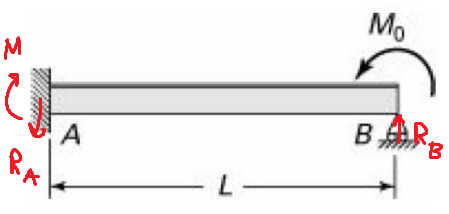
\includegraphics[width=0.5\linewidth]{Questions/Figures/Q2ProblemDiagram.png}
    \caption{Beam supported and loaded as shown.}
    \label{fig:Q2ProblemDiagram}
\end{figure}

The moment equation from B to A is:
\begin{align*}
    M &= R_B x + M_0 \\
    \frac{\partial M}{\partial R_B} &= x 
\end{align*}

By Castigliano's theorem,
\begin{align*}
    \delta_{B} &= \int_{0}^{L} \frac{M}{EI} \frac{\partial M}{\partial R_B} dx \\
    &= \int_{0}^{L} \frac{(R_B x + M_0)}{EI} (x) dx \\
    &= \frac{R_B L^3}{3EI} + \frac{M_0 L^2}{2EI} 
\end{align*}

There is a pin at B. It cannot carry and deflection. Therefore, $\delta_B = 0$. Solving for $R_B$,
\begin{align*}
    0 &= \frac{R_B L^3}{3EI} + \frac{M_0 L^2}{2EI} \\
    \implies R_B &= \frac{-3M_0}{2L} 
\end{align*}

The reaction at A has equal magnitude and opposite direction to $R_B$. Therefore,
\begin{equation*}
    \boxed{R_A = \frac{-3M_0}{2L}}
\end{equation*}

The moment at A is found by summing the moment about A:
\begin{align*}
    \sum M_A &= 0 \\
    &= -M + R_B L + M_0 \\
    \implies M &= R_B L + M_0 \\
    &= \frac{-3M_0}{2} + M_0 \\
    &= \boxed{\frac{-M_0}{2}} 
\end{align*}